\documentclass[12pt]{article}
\usepackage[utf8]{inputenc}
\usepackage{pifont}
\usepackage{tikz}
\usepackage{color}
\usepackage{graphicx}
\usepackage{indentfirst}

\begin{document}

\title{SAS para transportistas}

\section {Objetivo}
El objetivo principal de esta aplicación es que los transportistas valoren los viajes realizados para Batz S.Coop.
\section {Acceso al programa}
Para llegar al recurso se debe de acceder a la página https://xbi.batz.es
\par
Una vez aquí, se solicitan usuario y contraseña. En el caso de Azkar el usuario es: diego.rodriguez@azkar.com
\par
En la pantalla de menú principal, tenemos que seleccionar el icono SAS para que finalmente accedamos al programa.
\section {Funcionamiento del programa}
El programa mostrara todos los viajes realizados por Azkar para Batz S.Coop. Cada viaje tiene una casilla para insertar el precio del viaje y otra casilla para los comentarios. 
\section {Imagenes}
\fbox{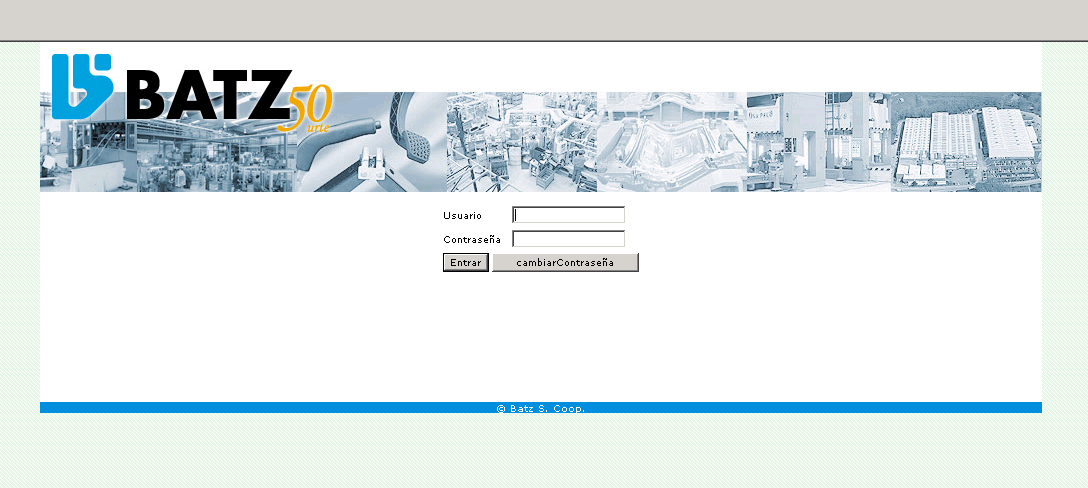
\includegraphics[width=15cm]{extranet_login.png}}
\par
\fbox{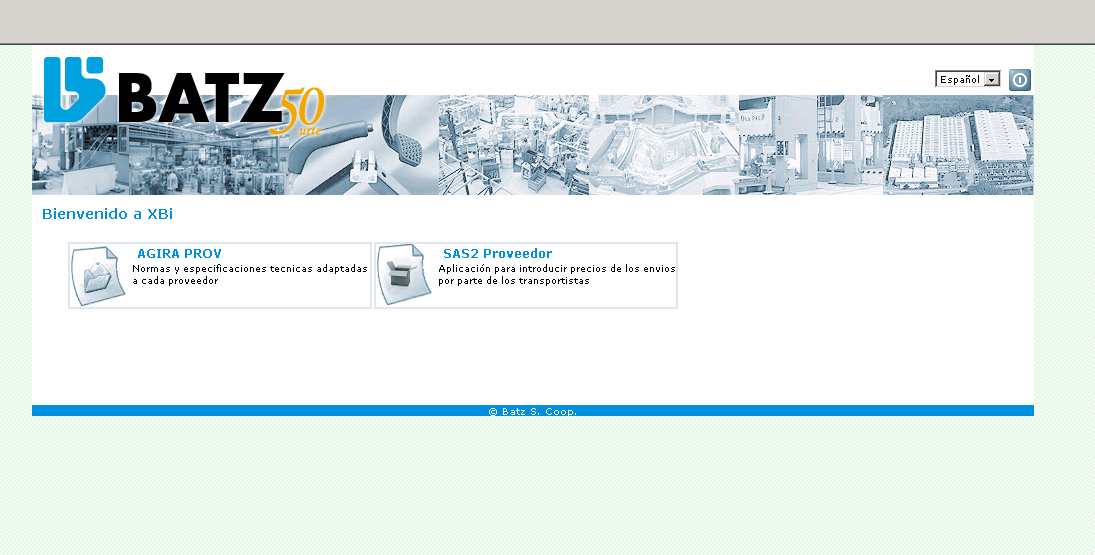
\includegraphics[width=15cm]{extranet_menu.png}}
\par
\fbox{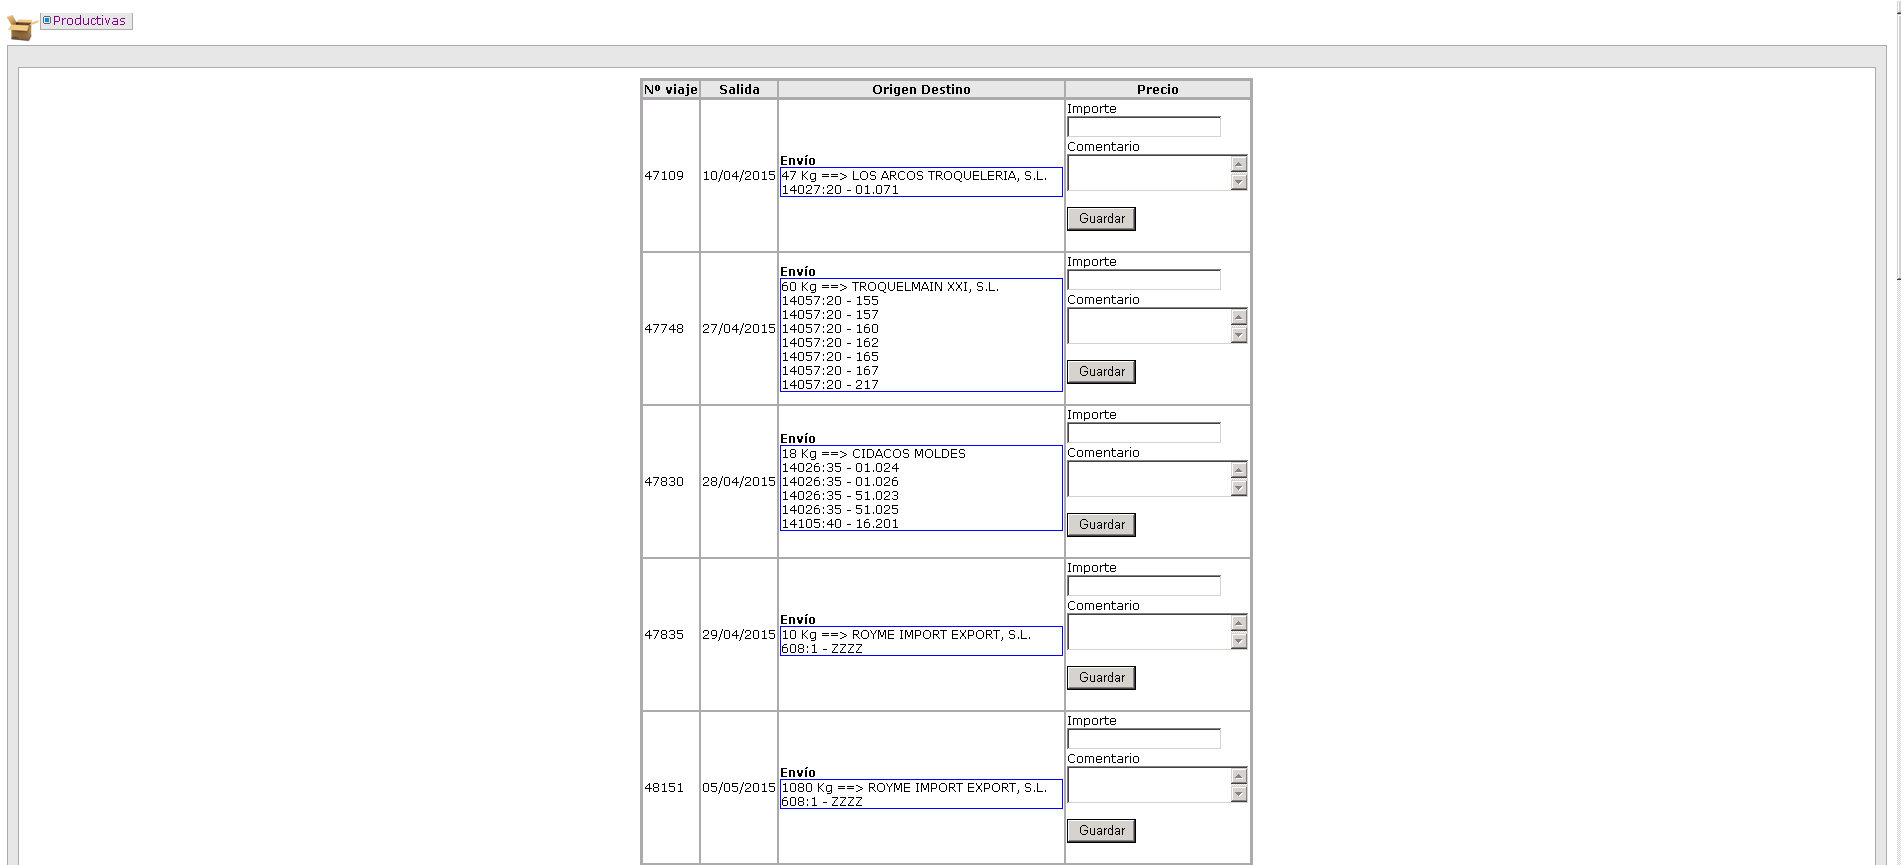
\includegraphics[width=15cm]{extranet_sas2.png}}
\end{document}


